\id{IRSTI 61.01.11}{}

{\bfseries ANALYSIS OF METHODS TO IMPROVE THE STRENGTH AND HEAT RESISTANCE}

{\bfseries OF COMPOSITE MATERIALS}

{\bfseries L.
Tolymbekova}
\begin{figure}[H]
	\centering
	
\includegraphics[width=0.8\textwidth]{media/chem/image1}
	\caption*{}
\end{figure}

{\bfseries , A.
Kolpek}
\begin{figure}[H]
	\centering
	
\includegraphics[width=0.8\textwidth]{media/chem/image1}
	\caption*{}
\end{figure}
{\bfseries ,
E.
Kopishev}
\begin{figure}[H]
	\centering
	
\includegraphics[width=0.8\textwidth]{media/chem/image1}
	\caption*{}
\end{figure}
{\bfseries ,
A.
Tursynova}
\begin{figure}[H]
	\centering
	
\includegraphics[width=0.8\textwidth]{media/chem/image1}
	\caption*{}
\end{figure}
{\bfseries \textsuperscript{\envelope },
G.
Seitenova}
\begin{figure}[H]
	\centering
	
\includegraphics[width=0.8\textwidth]{media/chem/image1}
	\caption*{}
\end{figure}
{\bfseries \textsuperscript{\envelope }}

L.N. Gumilev Eurasian National University, Astana, Kazakhstan

{\bfseries \textsuperscript{\envelope }}Corresponding author:
\href{mailto:tursynova_ak@enu.kz}{\nolinkurl{tursynova\_ak@enu.kz}},
\href{mailto:seitenova_gzh@enu.kz}{\nolinkurl{seitenova\_gzh@enu.kz}}

Modern composites occupy an important place in the production of
high-strength materials due to their lightness, strength, heat
resistance, ability to retain their performance properties and the
possibility of modification for certain tasks. The article presents
modern methods of improving mechanical properties and heat resistance of
metal and polypropylene-based composites, their key characteristics, as
well as modern processing technologies and innovative combinations with
other materials. Particular attention is paid to the prospects for the
development of composites with high temperature resistance through the
introduction of reinforcing refractory particles, the use of carbon
fibers and nanotubes, phosphorus-containing flame retardants, lignin,
elastomers, thermoplastics, which opens up new opportunities for their
exploitation.

Modification of polypropylene using various fillers, such as polyamides,
chalk fillers, and carbon nanoparticles, significantly improves its
performance characteristics, including strength, thermal stability, and
electrical conductivity. This opens up new horizons for the use of
polypropylene composites in conditions of high loads and high
temperatures, which is important for the sustainable development of the
electronics industry and other high-tech areas.

Metal and polypropylene-based composites have the potential for
application in high temperatures and aggressive environments due to the
possibility of modifying their structure and composition. The methods
and technologies presented in the article allow expanding their
functional capabilities, including integration with innovative
components.

{\bfseries Keywords:} composite materials, heat resistance, polypropylene,
nanocomposites, carbon nanotubes, fibers, thermoplastic elastomers,
adhesion.

{\bfseries АНАЛИЗ МЕТОДОВ ПОВЫШЕНИЯ ПРОЧНОСТИ И ТЕРМОСТОЙКОСТИ
КОМПОЗИЦИОННЫХ МАТЕРИАЛОВ}

{\bfseries Л. Толымбекова, А. Колпек, Е. Копишев, А. Турсынова
\textsuperscript{\envelope } , Г. Сейтенова \textsuperscript{\envelope },}

Евразийский национальный университет им. Л. Н. Гумилева, Астана,
Казахстан,

e-mail: tursynova\_ak@enu.kz,
\href{mailto:seitenova_gzh@enu.kz}{\nolinkurl{seitenova\_gzh@enu.kz}}

Современные композиты занимают важное место в производстве высокопрочных
материалов благодаря их легкости, прочности, термостойкости, способности
сохранять свои эксплуатационные свойства и возможности модификации под
определенные задачи. В статье представлены современные методы улучшения
механических свойств и термостойкости композитов на основе металла и
полипропилена, их ключевые характеристики, а также современные
технологии обработки и инновационные сочетания с другими материалами.
Особое внимание уделяется перспективам разработки композитов с высокой
термостойкостью за счет введения армирующих тугоплавких частиц,
использования углеродных волокон и нанотрубок, фосфорсодержащих
антипиренов, лигнина, эластомеров, термопластов, что открывает новые
возможности для их эксплуатации.

Модификация полипропилена с использованием различных наполнителей, таких
как

эксплуатационные характеристики, включая прочность, термическую
устойчивость и электрическую проводимость. Это открывает новые горизонты
для применения полипропиленовых композитов в условиях повышенных
нагрузок и высоких температур, что имеет важное значение для устойчивого
развития электронной промышленности и других высокотехнологичных
областей.

Композиты на основе металлов и полипропилена имеют потенциал для
применения в условиях высоких температур и агрессивных сред благодаря
возможности модификации их структуры и состава. Представленные в статье
методы и технологии позволяют расширить их функциональные возможности, в
том числе за счет интеграции с инновационными компонентами.

{\bfseries Ключевые слова:} композиционные материалы, термостойкость,
полипропилен, нанокомпозиты, углеродные нанотрубки, волокна,
термопластичные эластомеры, адгезия.

{\bfseries КОМПОЗИЦИЯЛЫҚ МАТЕРИАЛДАРДЫҢ БЕРІКТІГІ МЕН ЫСТЫҚҚА}

{\bfseries ТӨЗІМДІЛІГІН АРТТЫРУ ӘДІСТЕРІН ТАЛДАУ}

{\bfseries Л. Толымбекова, А. Көлпек, Е. Копишев, А.
Турсынова\textsuperscript{\envelope }, Г. Сейтенова\textsuperscript{\envelope }}

Л.Н. Гумилев атындағы Еуразия ұлттық университеті, Астана, Қазақстан,

e-mail: tursynova\_ak@enu.kz, seitenova\_gzh@enu.kz

Заманауи композиттер жоғары беріктігі бар материалдарды өндіруде маңызды
орын алады, олардың жеңілдігі, беріктігі, ыстыққа төзімділігі, пайдалану
қасиеттерін сақтау қабілеті және белгілі бір міндеттерге өзгерту
мүмкіндігі. Мақалада металл және полипропилен негізіндегі Композиттердің
механикалық қасиеттері мен ыстыққа төзімділігін жақсартудың заманауи
әдістері, олардың негізгі сипаттамалары, сондай-ақ заманауи өңдеу
технологиялары және басқа материалдармен инновациялық комбинациялар
ұсынылған. Арматуралық отқа төзімді бөлшектерді енгізу, көміртекті
талшықтар мен нанотүтіктерді, құрамында фосфор бар отқа төзімді заттар,
лигнин, эластомерлер, термопластиктерді қолдану арқылы жоғары
температураға төзімді композиттерді әзірлеу перспективаларына ерекше
назар аударылады, бұл оларды пайдаланудың жаңа мүмкіндіктерін ашады.

Полипропиленді полиамидтер, бор толтырғыштары және көміртекті
нанобөлшектер сияқты әртүрлі толтырғыштарды қолдану арқылы өзгерту оның
беріктігін, термиялық тұрақтылығын және электр өткізгіштігін қоса
алғанда, оның өнімділігін айтарлықтай жақсартады. Бұл электронды
өнеркәсіптің және басқа да жоғары технологиялық салалардың тұрақты дамуы
үшін маңызды болып табылатын жоғары жүктемелер мен жоғары температура
жағдайында полипропилен композиттерін қолданудың жаңа көкжиектерін
ашады.

Металдар мен полипропилен негізіндегі Композиттердің құрылымы мен
құрамын өзгерту мүмкіндігіне байланысты жоғары температура мен
агрессивті ортада қолдану мүмкіндігі бар. Мақалада ұсынылған әдістер мен
технологиялар олардың функционалдығын, соның ішінде инновациялық
компоненттермен интеграциялау арқылы кеңейтуге мүмкіндік береді.

{\bfseries Түйін сөздер:} композициялық материалдар, ыстыққа төзімділік,
полипропилен, нанокомпозиттер, көміртекті нанотүтікшелер, талшықтар,
термопластикалық эластомерлер, адгезия.

{\bfseries Introduction.} Modern industry is placing increasingly stringent
demands on materials, especially in areas such as automotive, aerospace
and construction. Traditional materials such as pure metal, plastic or
carbon often cannot meet the requirements for a combination of
lightness, strength and resistance to extreme temperatures. Composite
materials bring out the best properties of different components with
unique characteristics. Improving the mechanical properties and thermal
resistance of composites such as polypropylene, metal and carbon fiber
composites is an important factor in expanding their application and
performance.

Composites are materials made up of two or more components depending on
the natural conditions to achieve a unique advantage. The most widely
used types of composites include polymer, metal and carbon composites.
However, their performance properties are often limited by fragility,
insufficient heat resistance, or poor adhesion between phases {[}1-2{]}.

The main components of composites include matrix (base), responsible for
bonding and dependence, and reinforcing material (filler), increasing
strength and mechanical performance. At the present stage of industrial
development, composites are widely used in a wide variety of fields such
as construction, metallurgy, transportation, medicine, electronics, etc.
{[}3-6{]} The list of main types of composites is diverse and wide.
These are reinforced polymers, composites for pipelines and fittings,
metal matrix composites (MMC), heat resistant composites, carbon fiber
and glass fiber composites, biocomposites, materials for surgical
instruments, etc. {[}7-10{]}.

Current composites have their own problems and limitations, which
includes insufficient interfacial adhesion, brittleness under impact
loading, limited thermal resistance, difficulty in processing and
disposal, initial cost, lack of liquidity data, difficulty in developing
hybrid materials and lack of uniform standard qualities {[}11-13{]}.

Solving these problems requires a comprehensive solution, including the
development of new technologies, optimizing production processes,
improving environmental friendliness and reducing the cost of materials.

Despite this, composites remain in demand due to their excellent
properties, such as high strength, lightness, corrosion resistance and
the ability to create products with specified performance
characteristics. Constant development of technologies, development of
new types of composites and improvement of methods of their production
allow to regulate the scope of their application, reduce costs and
eliminate possible problems.

{\bfseries Materials and methods.} \emph{Metal-based composites.}
Metal-based composites attract great interest. Their structure, which
combines a metallic matrix with inclusions of non-metallic nature,
allows them to overcome the boundaries of high strength, lightness,
corrosion resistance and other unique properties unattainable for
traditional materials. Such properties make them in demand in various
industries including aerospace, automotive, energy and construction
sectors {[}14-16{]}. The most common matrices are aluminum, magnesium,
titanium, and iron. Reinforcing materials can be ceramic particles,
fibers, carbon nanostructures and oxide compounds.

One of the main advantages of metal composites is the ability to
fine-tune their properties by changing their composition and structure.
This is a way to optimize synthesis processes such as powder metallurgy,
mechanical alloying, reinforcement casting and additive technologies.
For example, the addition of carbon nanotubes to an aluminum matrix can
increase the density of a strong material without significantly
increasing its mass {[}17-19{]}.

Special attention is paid to the study of mechanical, thermal and
electrical properties of metal composites, as well as their behavior
under extreme operating conditions. Studies of thermal resistance and
durability open new horizons for the application of materials in
aggressive environments or at high temperatures {[}20-21{]}.

One of the promising structural materials with improved characteristics
are materials obtained by means of various types of reinforcement, such
as metal matrix CMs (composite materials) consisting of a metal or alloy
as a continuous matrix and a reinforcing component in the form of
particles, as well as short or continuous fibers {[}22-26{]}. In metal
matrix CM, the main metal matrices are aluminum, titanium, copper, and
magnesium alloys. According to literature data, in CMs with aluminum
matrix reinforced with carbon fiber, wetting of fibers is carried out to
a sufficient extent, which can improve mechanical properties
{[}27-30{]}.

Metal composites based on titanium matrix have high specific strength
and elastic modulus, high temperature resistance and low density, which
makes them attractive for aerospace, automotive and military
applications, but the use of titanium alloys as structural materials
under conditions of high friction and wear is limited due to their low
tribological properties {[}31-32{]}. Nevertheless, the addition of
refractory particles to titanium and its alloys is an effective way to
improve mechanical and wear properties.

The paper {[}33{]} presents studies on fabrication and evaluation of the
effect of the content of various reinforcing elements on the properties
of metal composite materials (MCMs) based on titanium alloys.
Introduction of refractory particles TiB\textsubscript{2},
B\textsubscript{4}C, SiC and TiC into titanium and its alloys is an
effective way to increase mechanical, wear-resistant and
corrosion-resistant properties with simultaneous reduction of material
density, and also contributes to the expansion of the area of
application of MCMs. The size and distribution of reinforcing particles
in the matrix and their chemical activity have a great influence on the
microstructure and mechanical properties. Carrying out heat treatment
process helps to increase the mechanical properties. Metal composites
reinforced with solid particles have an advantage (compared to MCMs
reinforced with continuous fibers) in the form of isotropic properties,
are cheaper to produce and can be further processed.

In {[}34{]}, the compound B\textsubscript{4}C was used as a reinforcing
element to improve the mechanical, corrosion, and tribological
properties of the titanium alloy of the composition Ti-6Al-4V
(hereinafter referred to as the alloy composition in \% (by mass)),
noting its thermodynamic stability and high mechanical properties. The
alloy of composition Ti- 6Al-4V and ceramic powder B\textsubscript{4}C
with an average particle size of 30 microns were used for the production
of MCM samples by powder metallurgy. MCM samples were made with the
content of 5 and 10 \% (by mass) of B\textsubscript{4}C. As a result of
the study of physical and mechanical properties of the samples, it was
found that the density of MCM decreases with increasing content of
reinforcing particles, but the difference between theoretical and
experimental density increases with increasing B\textsubscript{4}C
content, which is explained by the increase in porosity with increasing
content of B\textsubscript{4}C particles (Fig.1, a). The hardness and
corrosion resistance increase with increasing amount of reinforcing B4C
particles (Fig.1, b).

%% \begin{longtable}[]{@{}
%%   >{\raggedright\arraybackslash}p{(\linewidth - 0\tabcolsep) * \real{1.0000}}@{}}
%% \toprule\noalign{}
%% \begin{minipage}[b]{\linewidth}\raggedright
%% {\bfseries } experimental density {\bfseries } theoretical density
%% {\bfseries } porosity
%% \end{minipage} \\
%% \midrule\noalign{}
%% \endhead
%% \bottomrule\noalign{}
%% \endlastfoot
%% \end{longtable}

%% \begin{longtable}[]{@{}
%%   >{\raggedright\arraybackslash}p{(\linewidth - 8\tabcolsep) * \real{0.0470}}
%%   >{\raggedright\arraybackslash}p{(\linewidth - 8\tabcolsep) * \real{0.3946}}
%%   >{\raggedright\arraybackslash}p{(\linewidth - 8\tabcolsep) * \real{0.1152}}
%%   >{\raggedright\arraybackslash}p{(\linewidth - 8\tabcolsep) * \real{0.0470}}
%%   >{\raggedright\arraybackslash}p{(\linewidth - 8\tabcolsep) * \real{0.3962}}@{}}
%% \toprule\noalign{}
%% \begin{minipage}[b]{\linewidth}\raggedright
%% density g/cm3
%% \end{minipage} & \begin{minipage}[b]{\linewidth}\centering
%% 
\begin{figure}[H]
	\centering
	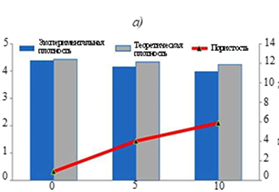
\includegraphics[width=0.8\textwidth]{media/chem/image6}
	\caption*{}
\end{figure}

%% \end{minipage} & \begin{minipage}[b]{\linewidth}\raggedright
%% density \%
%% \end{minipage} & \begin{minipage}[b]{\linewidth}\raggedright
%% hardness HV
%% \end{minipage} & \begin{minipage}[b]{\linewidth}\centering
%% 
\begin{figure}[H]
	\centering
	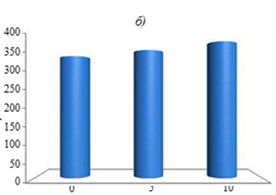
\includegraphics[width=0.8\textwidth]{media/chem/image7}
	\caption*{}
\end{figure}

%% \end{minipage} \\
%% \midrule\noalign{}
%% \endhead
%% \bottomrule\noalign{}
%% \endlastfoot
%% & particle content В\textsubscript{4}С, \% (by mass) & & & particle
%% content В4С, \% (by mass) \\
%% \end{longtable}

{\bfseries Fig.1 - Effect of the content of ceramic B\textsubscript{4}C
particles on the properties of MCM composition}

{\bfseries (Ti-6Al-4V) + B\textsubscript{4}C on density (a) and hardness
(b) {[}34{]}}

Similar studies {[}35-37{]} confirmed that the wear rate of the
composite material decreases with increasing in situ formed TiB and TiC
particles, and concluded that TiB and TiC particles improve the wear
properties of the composite material.

The influence of sintering temperature and the content of
B\textsubscript{4}C particles on the properties of composite material
obtained by powder metallurgy was investigated in {[}38{]}. The increase
in hardness and compressive strength of the composite material increases
with increasing sintering temperature and increasing the content of
reinforcing component.

In {[}39{]} the influence of B\textsubscript{4}C particles and laser
energy density on microhardness of composite material of Ti-6Al-4V
composition obtained by selective laser sintering was investigated. When
obtaining the composite material, B\textsubscript{4}C particles react
with titanium and in the in situ process TiC and TiB particles are
formed in different proportions, the microhardness increases by 30-80 \%
depending on the laser energy density.

Currently, high-modulus carbon fibers are the most suitable material for
creating composites with titanium matrix. Selective reinforcement of
titanium plates of small thickness allows to provide control of high
reactivity of "titanium/carbon" compound and to create suitable
processing methods {[}40-42{]}.

Laminated structures consisting of alternating layers of metal sheets
and fiber-reinforced polymer-matrix composites are also used in aircraft
parts structures. Compared to conventional monolithic metals, they have
high specific strength and stiffness, excellent fatigue resistance
characteristics, and increased fire resistance {[}43{]}.

To improve the mechanical properties of CMs with layered structure,
including metal plastic layer and intermetallic layer (Ti-Al3Ti),
various continuous fibers - carbon (C), silicon carbide (SiC) and
aluminum oxide (Al\textsubscript{2}O\textsubscript{3}) - are introduced.
Using various processing techniques, a number of intermetallic metallic
layered CMs of systems such as Ti-Al, Ni-Al, Nb-Al and Ti-Cu are
obtained. It is believed that the application of such titanium-aluminum
layered CMs with high physical and mechanical properties is potentially
possible in aerospace and armor protection applications. Using a novel
rapid prototyping technique, ultrasonic consolidation was applied to
fabricate three-dimensional structures via additive manufacturing from
metal foil. During the ultrasonic consolidation process, ultrasonic
frequency vibration combined with nominal force was used to generate
static and oscillating shear forces between the metal foil layers that
formed a solid-state bond. Moreover, ultrasonic consolidation was used
to join dissimilar materials such as Ti-Al, Cu-Al, and Fe-Al at low
temperatures (\textasciitilde480 °C). Thus, ultrasonic consolidation can
be used as an auxiliary method to disperse fiber bundles into individual
fibers in the alloy matrix prior to CM formation {[}44-46{]}.

In {[}47{]}, studies were conducted to determine the mechanical
characteristics of CM produced by die casting method using AA6061 matrix
aluminum alloy, which is reinforced with carbon fiber. The studies
showed that increasing the content of reinforcing component from 0 to
10\% (vol.) allows increasing the torque from 24.5 to 52 N-m, tensile
strength from 283 to 315.5 MPa, as well as increasing the impact
strength at 10\% (vol.) of carbon fiber up to 12.2 J {[}47{]}.

The microstructure of the CM of AA6061 grade aluminum alloy and carbon
fiber shows that the carbon fibers are evenly distributed in the matrix,
and interfacial adhesion is present (Figure 2).


\begin{figure}[H]
	\centering
	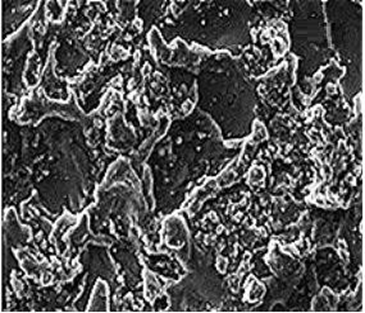
\includegraphics[width=0.8\textwidth]{media/chem/image8}
	\caption*{}
\end{figure}


{\bfseries Fig.2 - Microstructure of composite material made of aluminum
alloy}

{\bfseries AA6061 and carbon fiber {[}47{]}}

In similar works {[}48-50{]} the authors describe in detail the physical
and mechanical characteristics of materials with different matrix alloys
(content of reinforcing carbon fibers - from 5 to 50 \% (vol.)) and the
mechanisms of failure of composites after the tests. In {[}48-49{]},
studies of thermophysical and mechanical properties of CMs obtained by
powder metallurgy on the basis of aluminum matrix reinforced with carbon
fibers were carried out. It was found that when the volume content of
carbon fiber increases, hardness, electrical conductivity and strength
decrease: from 71 to 56 HB, from 30.9 to 14.5 cm and from 529 to 214
MPa, respectively, thermal conductivity increases to 155 W/(m-K), and
the temperature coefficient of linear expansion (TCLE) decreases - from
36-10-6 to 8-10-6 K-1 {[}48{]}.

Among the basic properties of composite materials, heat resistance and
heat resistance, the ability of a material to retain its original
strength at high temperature, are of particular importance for the most
common structures {[}51-53{]}. For other types of heat-resistant
materials, such as those based on minerals (ceramics, refractories with
various mineral fillers and binders), the concept of refractoriness is
applicable, i.e. the ability of the material to resist destruction
without deforming during operation at temperatures not lower than 1580
°C {[}54{]}. Composite materials with ceramic matrix have high heat
resistance, relatively high compressive strength, but tensile strength
and impact strength have low values. The scientific direction of solving
the problem of increasing the strength of composite material is the
necessity of transferring a significant part of the load to reinforcing
elements {[}55-57{]}.

It is of scientific and practical interest to solve the problem of
increasing the strength and heat resistance of composite material of the
metal-ceramic system by changing the macrostructure of the introduced
reinforcing material and matrix composition.

The most common methods of molding composite materials are pressing and
sintering, which in some cases is not economical, for example, molds are
difficult to manufacture, this disadvantage significantly increases the
cost of products. The use of slurry with hydrophilic tooling to remove
moisture and give primary technological strength to the composite
material, provides cost reduction and increased cost-effectiveness
{[}58-60{]}.

In work {[}61{]}, the analysis of properties of composite materials is
given, increase of heat resistance and heat resistance of composite
material on the basis of stabilized silica, wastes of metallurgical and
glass industries, was achieved by improving the structure of composite
material, introduction of reinforcing elements. For the production of
composite material was used an economical method of molding into
hydrophilic tooling.

Slip is a suspension in the form of liquid dispersion medium and solid
fine-dispersed phase, for example, in the form of SiO2 and Fe, crushed
to the size of 0.5...10 microns, as well as additives: stabilizing
volumetric transformations of SiO2 during heating or cooling (Na2O);
increasing sedimentation stability of slip (refractory clay). This
material is fluid in the stage of preparation and pouring, plasticity
while in the mold and strength after partial dehydration of the slip,
for example, in a gypsum mold. The combination of stabilized
silica-based slurry, reinforcing components, glass production waste and
hydrophilic tooling reduces energy consumption by 18\% and increases the
cost-effectiveness of manufacturing products of the metal-ceramic system
in comparison with traditional methods of composite materials forming
{[}61{]}.

Despite the obvious advantages, the development of metal-based
composites involves obtaining a criterion for uniform distribution of
reinforcing particles and the need to accurately determine the
interactions between components. However, modern advances in computer
modeling, nanotechnology, and experimental techniques offer new
opportunities to overcome these difficulties. Thus metal-based
composites continue to be the basis of research that will shape the
development of high-tech materials in the future. Their unique
properties and potential applications in a wide range of regions make
them the object of close attention of the scientific community and
industry.

\emph{Polypropylene-based composites.} Today, polymer composites are of
particular interest and are being actively introduced into various
fields due to their unique properties, including high elasticity,
strength, stiffness and high specific strength.

Polypropylene is one of the most widely used polymers in the world.
Since its commercial introduction in the 1950s, polypropylene has
established a reputation for its unique properties and versatility in
application {[}62{]}.

Polypropylene can be easily molded and extruded to produce complex
shapes. It is able to retain its size and shape when exposed to high
temperatures and loads. It combines low density and high strength,
making it ideal for use in the manufacture of lightweight but strong
products {[}63{]}.

Modern technologies make it possible to combine polypropylene with
natural and synthetic fibers. This opens up new possibilities for
creating materials with improved thermal and mechanical properties. The
addition of synthetic fibers and fillers (such as carbon or glass
fibers) can improve the strength and stiffness of polypropylene
products, which expands their application {[}64{]}.

The improvement of these materials through the addition of carbon
nanotubes (CNTs) and fibers is an active area of research aimed at
improving their performance {[}65{]}.

Modification of polypropylene with carbon nanotubes and fibers allows to
significantly improve the mechanical properties of composites, in
particular, their impact resistance and stiffness. It was found that the
addition of carbon nanotubes can increase the impact resistance of the
composite up to seven times, which makes such materials competitive with
more expensive analogs. Mechanical stiffness and resistance to
deformation under load are also significantly increased by the inclusion
of continuous carbon fibers, which expands their application areas,
including high and low temperature conditions {[}66{]}.

The need to use carbon nanotubes arises due to their unique properties,
including high thermal conductivity, strength and the ability to form
conductive networks within the polypropylene structure. Studies show
that the introduction of CNTs into PP composites leads to a significant
improvement in mechanical properties due to a more homogeneous
distribution of reinforcing additives and their strong interaction with
the polymer matrix {[}67{]}.

Many CNT modification techniques, including covalent and non-covalent
modification, are used to achieve the best results in the creation of
composites. These methods help to improve the dispersion of fillers in
the polymer matrix, allowing for more robust interfacial interactions.
CNT modification allows the attachment of functional groups such as
epoxy, hydroxyl and carboxyl groups, which also helps to improve the
bond strength between the matrix and filler {[}68{]}.

In addition, oxidation of carbon nanotubes carried out using various
oxidizing agents such as H₂SO₄, KMnO₄, H₂O₂ and HNO₃ allows the
introduction of functional groups on their surface. This leads to the
formation of defective sites, which can adversely affect the engineering
properties, but this approach significantly improves the adhesion of
CNTs in the polymer matrix, which is the cornerstone of an efficient
composite structure {[}69{]}.

The introduction of nanotubes into the structure of polypropylene
composites provides improvements in properties such as strength, heat
resistance and mechanical stiffness, making them competitive with more
expensive materials {[}70{]}.

Studies show that PP and nanotube-based composites exhibit significant
improvements in mechanical properties such as impact resistance and
stiffness. Carbon nanotubes contribute to increased strength and
resistance to deformation under loading due to their high strength and
ability to form conductive networks within the polymer matrix. In
particular, the use of metallocene polypropylene in combination with
carbon fillers improves the strength and ductility of composites
{[}71{]}.

Melt extrusion is the preferred method of producing PP-CNT composites
because of its ability to create homogeneous materials through mixing of
components at high temperatures. However, lack of control during the
extrusion process can lead to thermal fracture and residual stresses
that negatively affect the properties of the composites. To increase the
dispersion of CNTs in the polymer matrix, various modifications and
blending methods are actively investigated, indicating the importance of
controlling the extrusion process to achieve optimal performance
{[}72{]}.

Modifications of carbon nanotubes are necessary to ensure high-quality
interfacial adhesion between PP and CNTs. The grafting of maleic
anhydride (MA) onto polymer chains significantly improves the
compatibility of CNTs with the polymer matrix and also helps to reduce
the surface tension. This allows for better dispersion of CNTs and
formation of efficient percolation networks. Studies show that the use
of modified compatibilizers such as styrene-ethylene/butylene-styrene
copolymer leads to a significant improvement in the mechanical and
thermal properties of composites {[}73{]}.

The high flammability of polypropylene limits its use in applications
requiring fire resistance. To solve this problem, active research is
directed to the use of phosphorus-containing flame retardants
(phosphorus fire retardant additives), which show high efficiency in
reducing the flammability of polymeric materials {[}74{]}.

Phosphorus flame retardants have unique properties that provide low
toxicity and the ability to form a protective layer on the surface of
the material when exposed to high temperatures. This protective layer
promotes thermal decomposition of the flame retardant, forming a carbon
residue that serves as a barrier to flame propagation. These mechanisms
of action make it possible to significantly increase the fire resistance
of polypropylene composites {[}75{]}.

Studies conducted by various research groups have confirmed that the
addition of phosphorus flame retardants to PP significantly improves its
mechanical and thermal properties. The addition of phosphorus flame
retardants to PP increases the tensile strength and stiffness of
composites at high temperatures, which improves their performance
without degrading the basic properties {[}76{]}.

Phosphorus-containing flame retardants are a promising alternative to
halogen-containing flame retardants, which were previously widely used
but criticized for their toxicity and negative environmental impact. In
contrast, phosphorus-containing additives help to reduce flammability
while remaining safer for humans and nature {[}77{]}.

The retrofitting of polypropylene with phosphorus-containing flame
retardants opens new horizons for the application of composites in
products that require high fire resistance. For example, the study of
new methods of modifying composites, such as blending with carbon
nanotubes (CNTs), improves thermal stability and mechanical properties
while maintaining environmental safety {[}78{]}.

To achieve higher performance characteristics of polypropylene
composites with phosphorus-containing flame retardants, it is necessary
to continue the optimization of compositions and technologies of their
processing. This includes the study of new polymer modifications and the
use of alternative fillers, which can lead to the creation of stable and
functional materials that meet modern requirements {[}79{]}.

Polypropylene is one of the most popular thermoplastics with good
mechanical and physical properties. However, various modification
methods are being investigated to enhance its functionality and
performance, including the use of biopolymers such as lignin and
chitosan. These additives not only improve the mechanical properties of
composites but also make them more environmentally friendly {[}80{]}.

Modification of polypropylene with chitosan fibers can significantly
improve its strength and impact resistance. Chitosan, being a biopolymer
with good adhesion to the polymer matrix, contributes to the improvement
of tensile and impact performance. Experiments have demonstrated that
composites with modified fibers provide a significant improvement in
mechanical properties compared to unmodified samples {[}81{]}.

The use of esterified lignin as a modifier is important for achieving
high adhesion between composite components. Lignin, being a secondary
natural polymer, shows excellent binding properties, which improves the
structure of the final material. Studies show that the presence of
lignin helps to create strong interfacial interactions between chitosan
and polypropylene, which enhances the strength and durability of the
composite {[}82{]}.

The process of mixing the components at high temperatures, such as
190°C, ensures uniform distribution of fillers in the polypropylene
matrix. Homogeneity of distribution is critical to achieving optimum
strength and strain resistance. Studies in this area show that lack of
homogeneity can lead to poor mechanical performance and reduced material
stability {[}83{]}.

The resulting polypropylene-based composites with modifiers such as
lignin and chitosan have a wide range of potential applications in
industries such as packaging and construction. These fields require
lightweight and strong materials that can withstand mechanical stresses.
The improved performance of modified composites opens up new
opportunities for their use in various sectors including automotive and
consumer products {[}84{]}.

Composites based on thermoplastic elastomers have attracted considerable
attention due to their unique properties that provide high flexibility,
strength and resistance to external influences. Of particular interest
is the combination of styrene thermoplastic elastomers with
polypropylene, which makes them promising for applications in the
construction industry and other areas where high strength and durability
of materials are required {[}85{]}.

Thermoplastics are classes of polymers that combine the properties of
thermoplastics and elastomers. They are recyclable, making them
convenient for manufacturing processes, while providing the elasticity
characteristic of rubber bands. Studies show that blends of styrene
thermoplastic elastomers and polyolefin elastomers can improve the
performance of materials, which has initiated a number of scientific
studies in this area {[}86{]}.

One of the key tasks in improving composites based on thermoplastic
elastomers is to increase their resistance to thermal oxidative
degradation. Studies show that the introduction of antioxidants,
heat-resistant fillers and modifiers can significantly improve the
performance characteristics of materials and their durability {[}87{]}.

Improving the fire resistance of thermoplastic elastomers is also an
important aspect for their use in building structures. The use of
minerals such as aluminum hydroxide and other flame-retardant additives
shows promising results in improving the fire-retardant properties of
composites, making them safer for use in high temperature environments
{[}88{]}.

The problem of rubber waste utilization remains relevant, and the use of
crumb rubber as a filler for thermoplastics provides an opportunity not
only to solve environmental problems, but also to expand the application
area of such composites. Studies have proven that the addition of crumb
rubber to polyethylene and polypropylene can improve certain mechanical
characteristics such as impact strength and flexibility {[}89{]}.

The key factors affecting the mechanical properties of composites are
matrix characteristics, filler particle size and the level of adhesion
between components. Optimization of these properties can be achieved by
various methods such as changing the mixing technology, using modifiers
and adhesion promoters {[}90{]}.

The study of composites based on thermoplastic elastomers, particularly
their blends with polypropylene and styrene thermoplastic elastomers,
has become an important aspect because of the increasing demands for
durability and safety of building materials {[}91{]}.

Thermoplastic elastomers, including blends with polyolefin elastomers,
have flexible, strong and resistant properties. This allows them to find
applications in the construction, medical and automotive industries,
where high strength and durability of materials are required {[}92{]}.

Also the practical significance of the research lies in the development
of new formulations of composites based on thermoplastic elastomers,
which allows to create materials with improved performance
characteristics. The created composites are characterized by high
resistance to thermo-oxidative degradation and reduced flammability,
which makes them suitable for the production of window seals, cable
products, roofing membranes and other construction products {[}93{]}.

The introduction of crumb rubber into the composition of thermoplastics
solves the problems of utilization of waste rubber products and expands
the practical applications of plastics. The resulting rubber plastics
are used in waterproofing, production of roofing materials and rubber
tiles, while optimizing their mechanical properties {[}94{]}.

Studies show that different temperatures and rubber filler content
significantly affect the deformation and strength of composites. In
particular, certain concentrations of crumb rubber contribute to the
transition of the material from brittle fracture to macrouniform plastic
deformation, which opens up opportunities for targeted modification of
the properties of rubber plastics {[}95-96{]}.

Incorporation of waste-derived graphene into polymer composites can
increase their mechanical and thermal performance while improving
flexural and tensile strength. This supports the trend towards lighter
and greener materials, which helps to reduce the carbon footprint in the
automotive and other industries {[}97{]}.

{\bfseries Results and Discussion.} Research into polymers with improved
conductive properties opens new horizons for flexible electronics. The
development of conductive polymer nanocomposites can contribute to the
creation of more reliable and durable flexible electronic devices, which
will be a significant step forward in technology development {[}98{]}.

Modification of polypropylene using various fillers such as polyamides,
chalk fillers and carbon nanoparticles significantly improves its
performance characteristics including strength, thermal stability and
electrical conductivity. This opens new horizons for the application of
polypropylene composites in high stress and high temperature
environments, which is important for the sustainable development of the
electronics industry and other high-tech fields {[}99{]}.

Research and development of polypropylene-based nanocomposites using
various fillers open new horizons in the construction industry,
improving the mechanical characteristics and thermal stability of
materials. Special fillers help to accelerate crystallization processes
and increase resistance to environmental influences, which makes such
composites competitive for use not only in construction, but also in the
packaging and automotive industries {[}100{]}.

Thus, polypropylene composites are a promising area in materials
production due to their versatility, availability and modification
possibilities, such as carbon nanotubes, phosphorus-containing flame
retardants, lignin, elastomers, thermoplastics and others. These
modifications allow to significantly improve mechanical properties, heat
resistance, flame retardancy and expand their application in high-tech
and industrially important areas.

{\bfseries Conclusions.} Research in the field of increasing the strength
and heat resistance of composite materials is one of the promising areas
in the field of chemical technologies and materials science, opening up
wide opportunities for the development of innovative solutions.

Metal and polypropylene-based composites have the potential for
application in high temperatures and aggressive environments due to the
possibility of modifying their structure and composition. The methods
and technologies presented in the article allow expanding their
functional capabilities, including integration with innovative
components.

The review shows that the use of modern modification methods, such as
the introduction of reinforcing refractory particles, improvement of
interfacial interaction, the use of carbon fibers and nanotubes,
phosphorus-containing flame retardants, lignin, elastomers,
thermoplastics allows to significantly increase the strength
characteristics and heat resistance of composites.

The prospectivity of developments in this direction is due to the
growing requirements for materials used in the metallurgical industry,
construction, transportation, energy. Special attention should be paid
to the development of hybrid materials that combine the advantages of
polymers, metals and carbon fibers. Future research should be aimed at
optimizing upgrading technologies and studying their performance
characteristics of composites.

\emph{{\bfseries Funding:} BR24992883 Establishment of a science and
technology park for petrochemicals and polymer materials to provide
services and implementation of applied Research Work results in priority
sectors of the country' s economy (2024-2026).}

{\bfseries References}


1. Kolosova A.S., Sokolskaya M.K., Vitkalova I.A. Sovremennye polimernye
kompozicionnye materialy i ih primenenie // Mezhdunarodnyj zhurnal
prikladnyh i fundamental' nyh issledovanij. - 2018. --
No.5. -- S.245-256. {[}in Russian{]}

1. Lebedeva O.V., SipkinaE.I. Polimernye kompozity i ih svojstva //
Izvestija vuzov. Prikladnaja himija i biotehnologija. -- 2022. -- Tom
12. -- No.2. -- S.192-207. DOI 10.21285/2227-2925-2022-12-2-192-207.
{[}in Russian{]}

1. Gurbanov N.A., Sidorov D.B., Ismailova K.H. Composite materials,
general properties and usage areas // Sciences of Europe. -- 2021. --
No.78. -- P.25-27. DOI 10.24412/3162-2364-2021-78-1-25-27

1. Hull D., Clyne T.W. An Introduction to Composite Materials. --
Cambridge: Cambridge University Press.1996. -- 326 p. ISBN
978-0521388559. DOI 10.1017/CBO9781139170130

1. Schwartz M.M. Composite Materials: Properties, Non-Destructive Testing
and Repair, Polymer, Ceramic, Metal Matrices. -- USA: Prentice Hall
Inc., 1997. -- 423 p. ISBN-10 100133000478, ISBN-13 978-0133000474

1. Sumithra G., Reddy R., Kumar G, Ojha S., Jayachandra G., Raghavendra
G. Review on composite classification, manufacturing, and applications
// Materials Today: Proceedings. -- 2023. -- P.45-51. DOI
10.1016/j.matpr.2023.04.637

1. Ashrith H.S. , Jeevan T.P., Xu Jinyang. A Review on the Fabrication
and Mechanical Characterization of Fibrous Composites for Engineering
Applications // J. Compos. Sci. -- 2023.7, 252. DOI
10.3390/jcs7060252

1. Novye materialy {[}Tekst{]} / V.N. Anciferov {[}i dr.{]}; red. Ju.S.
Karabasov. - M.: MISIS, 2002. - 736 s. ISBN 5-87623-114-2. {[}in
Russian{]}

1. Resego~Phiri,~Sanjay~Rangappa,~Suchart~Siengchin. Advances in
lightweight composite structures and manufacturing technologies: A
comprehensive review// Heliyon. -- 2024. -- Vol.10, Issue 21. -- 24
p. DOI 10.20998/2074-272X.2017.6.01

1. Wanberg J. Composite Materials: Fabrication Handbook \#2. -- USA:
Wolfgang Publications, Inc., 2010. -- 144 p. ISBN 1929133936.

1. Jah' jaeva H.Sh., Zajkov G.E., Deberdeev T.R., Ulitin
N.V. Strukturnye osnovy mezhfaznoj adgezii v polimernyh kompozitah //
Vestnik Kazanskogo tehnologicheskogo universiteta. -- 2012. -- T.15.
-- No.5. -- S.68-70. {[}in Russian{]}

1. Smirnova O.E., Pichugin A.P., Hritankov V.F. Adgezionnaja
prochnost'{} v strukture kompozicionnyh materialov na
osnove organicheskogo syr' ja //
Stroitel' nye materialy. -- 2024. -- No.5. --S.17-21.
\href{https://doi.org/10.31659/0585-430X-2024-824-5-17-21}{DOI
10.31659/0585-430X-2024-824-5-17-21}. {[}in Russian{]}

1. Mel' nichenko M. A., Ershova O. V., Chuprova L. V.
Vlijanie sostava napolnitelja na svojstva polimernyh kompozicionnyh
materialov // Molodoj uchenyj. -- 2015. -- No.16 (96). -- S.199-202.
{[}in Russian{]}

1. Milejko S.T. Novye kompozity s metallicheskoj matricej //
Mezhotraslevoj seminar pamjati prof. T.D. Karimbaeva "Primenenie
kompozicionnyh materialov v dvigatelestroenii". Moskva, Rossija. --
2023. -- S.7-10. {[}in Russian{]}

1. Ivanov V.A. Metody vosstanovlenija tehnologicheskogo i
vspomogatel' nogo oborudovanija iznosostojkimi
kompozicionnymi materialami: diss. ... kand. tehn. nauk: 05.02.13 -
Mashiny, agregaty i processy (ljogkaja
promyshlennost'). -- Moskva. -- 2014. --166 s. {[}in
Russian{]}

1. Milejko S.T. Jentoni Kelli i kompozitnye materialy segodnja.
Chast'{} 2: Kompozity s metallicheskoj matricej //
Kompozity i nanostruktury.2021. --T.13. -- No.3-4 (51-52). -- S.
59-107. DOI 10.36236/1999-7590-2021-13-3-4-59-107. {[}in Russian{]}

1. Senjushkin N.S., Jamaliev R.R., Jalchibaeva L.R. Primenenie
kompozicionnyh materialov v konstrukcii bespilotnyh
letatel' nyh apparatov // Molodoj uchenyj.2011. --T.
1. -- No.4 (27).1. --S.59-61. {[}in Russian{]}

1. Even C., Arvieu C., Quenisset J.M. Powder route processing of carbon
fibers reinforced titanium matrix composites // Composites Science and
Technology. -- 2008. -- Vol.68(6). -- P.1273-1281. DOI
10.1016/j.compscitech.2007.12.014.

1. Saldias C., Bonardd S., Quezada C., Radic D., Leiva A. The role of
polymers in the synthesis of noble metal nanoparticles: a review //
Journal of Nanoscience and Nanotechnology. --2017. -- Vol.17. -- P.
87-114. DOI 10.1166/jnn.2017.13016

1. Prokopec A.D. Stroenie i mehanicheskie harakteristiki sloistogo
kompozicionnogo materiala na osnove MAH-fazy Ti₃AlC₂, poluchennogo
metodom svobodnogo SVS-szhatija / A.D. Prokopec, P.M. Bazhin, A.S.
Konstantinov, A P. Chizhikov, P.A. Stolin // Neorganicheskie
materialy. -- 2021. -- T.57. -- No.9. -- S.986--990. DOI
10.31857/S0002337X2109013X. {[}in Russian{]}

1. Sabadaha E.N., Prokopchuk N.R., Shutova A.L.
Termostabil' nye kompozicionnye materialy // Trudy
BGTU. -- 2017. -- Serija 2. -- No.2. -- S.108-115. {[}in Russian{]}

1. Grashhenkov D.V. Strategija razvitija nemetallicheskih materialov,
metallicheskih kompozicionnyh materialov i teplozashhity //
Aviacionnye materialy i tehnologii. -2017. - No. S. -S.264-271. DOI
10.18577/2071-9140 -2017-0-S-264-271. {[}in Russian{]}

1. Akmeev A.R., Guljaev I.N., Il' ichev A.V., Ivanov N.V.
Issledovanie mehanicheskih svojstv metallokompozita
(Aljuminij-ugleplastik) s adaptivnoj shemoj armirovanija //
Aviacionnye materialy i tehnologii. -- 2017. -- No.3 (48). -- S.
43-49. DOI 10.18577 /2071 -9140-2017-0-3-43-49. {[}in Russian{]}

1. Jakovlev A.L., Nochovnaja N.A., Putyrskij S.V., Krohin V.A.
Titanopolimernye sloistye materialy // Aviacionnye materialy i
tehnologii. -- 2016. -- No. S2 (44). -- S.56-62. DOI
10.18577/2071-9140-2016-0-S2-56-62. {[}in Russian{]}

1. Arislanov A.A., Goncharova L.Ju., Nochnaja N.A., Goncharov V.A.
Perspektivy ispol' zovanija titanovyh splavov v
sloistyh kompozicionnyh materialah // Trudy VIAM. -- 2015. -- No.10.
-- S.20-23. DOI 10.18577/2307-6046-2015-0-10-4-4. {[}in Russian{]}

1. Valueva M.I., Zelenina I.V., Haskov M.A., Guljaev A.I. Podgotovka
uglerodnogo volokna k naneseniju interfaznogo pokrytija dlja
kompozicionnyh materialov s keramicheskoj matricej// Trudy VIAM. --
2017. -- No.10 (58). -- S.79-89. DOI
10.18577/2307-6046-2017-0-10-9-9. {[}in Russian{]}

1. Bedmar J., Torres В., Rams J. Manufacturing of Aluminum Matrix
Composites Reinforced with Carbon Fiber Fabrics by High Pressure Die
Casting // Materials. -- 2022.15(9).3400. -- Р.2-18. DOI
10.3390/ma15093400

1. Jian-jun~Sha,~Zhao-zhao~Lü,~Ru-yi~Sha., et al. Improved wettability
and mechanical properties of metal coated carbon fiber-reinforced
aluminum matrix composites by squeeze melt infiltration technique //
Transactions of Nonferrous Metals Society of China. -- 2021. -- Vol.
31. Issue 2. -- P.317-330. DOI 10.1016/S1003-6326(21)65498-5

1. Lee Y., Park S., Han J. Carbon Fiber/Aluminum Composite Fabrication
Using Wettability Control // Composites Research. -- 2015. -- Vol.28.
Issue 5. -- P.254-259. DOI 10.7234/composres.2015.28.5.254

1. Choi Y., Meng Х., Xu Z. Manufacturing process of short carbon fiber
reinforced Al matrix with preformless and their properties //
Scientific Reports. -- 2021. -- 11:23385 -- P.1-8. DOI
10.1038/s41598-021-02915-7

1. Tian Y.S., Chen C.Z., Chen L.B., Liu J.H. Wear properties of alloyed
layers produced by laser surface alloying of pure titanium with
B\textsubscript{4}C and Ti mixed powders // Journal of Materials
Science. -- 2005. -- Vol.40. -- P.4387-4390. DOI
10.1007/s10853-005-0736-2

1. Fouvry S., Paulin C., Deyber S. Impact of contact size and complex
gross-partial slip conditions on Ti-6Al-4V/Ti-6Al-4V fretting wear //
Tribology International. -- 2009. -- Vol.42(3). -- P.461-474. DOI
10.1016/j.triboint.2008.08.005

1. Krasnov E.I., Serpova B.M., Hodykin L.F., Gololobov A.B.
Metallicheskie kompozicionnye materialy na osnove titanovyh splavov,
armirovannyh tugoplavkimi chasticami (Obzor) // Trudy VIAM. -- 2021.
-- No.6 (100). -- S.36-45. DOI 10.18577/2307-6046-2021-0-6-36-45.
{[}in Russian{]}

1. Soorya Prakash K., Gopal P.M., Anburose D., Kavimani V. Mechanical,
corrosion and wear characteristics of powder metallurgy processed
Ti-6Al-4V/B4C metal matrix composites // Ain Shams Engineering
Journal. -- 2018. -- Vol.9(4). -- P.1489--1496. DOI
10.1016/j.asej.2016.11.003

1. Qin Y.L., Geng L. Dry sliding wear behavior of titanium matrix
composites hybrid-reinforced by in situ TiB whisker and TiC particle
// Journal of Materials Science. -- 2011. -- Vol.46. -- P.4980-4985.
DOI 10.1007/s10853-011-5415-x

1. Balaji V.S., Kumaran S. Dry sliding wear behavior of titanium (TiB +
TiC) in situ composite developed by spark plasma sintering //
Tribology Transactions. -- 2015. -- Vol.58(4). -- P.698--703. DOI
10.1080/10402004.2014.993780

1. Zheng B., Dong F., Yuan X. et al. Microstructure and tribological
behavior of in situ synthesized (TiB + TiC)/Ti6Al4V (TiB/TiC = 1/1)
composites // Tribology International. -- 2020. -- Vol.145: 106177.
DOI 10.1016/j.triboint.2020.106177

1. Yoganandam K., Mohanavel V., Vairamuthu J, Kannadhasan V. Mechanical
properties of titanium matrix composites fabricated via powder
metallurgy method // Materials Today: Proceedings. -- 2020. --Vol.
33(7). -- P.3243-3247. DOI 10.1016/j.matpr.2020.04.569

1. Fereiduni E. Selective laser melting of hybrid ex-situ/in-situ
reinforced titanium matrix composites: Laser/powder interaction,
reinforcement formation mechanism, and non-equilibrium microstructural
evolutions / E. Fereiduni, A. Ghasemi, M. Elbestawi // Materials \&
Design. -- 2019. -- Vol.184:108185. DOI 10.1016/j.matdes.2019.108185

1. Peters M. Titanium Metal Matrix Composites: An Overview / Leyens C.,
Kumpfert C., Nickel R. B. // Composites Part A: Applied Science and
Manufacturing. -- 2019. -- Vol.121. -- P.418-438. DOI
10.1016/j.compositesa.2019.04.005

1. Arvieu, C. Interaction between titanium and carbon at moderate
temperatures {[}Text{]} / C. Arvieu, J.P. Manaud, J.M. Quenisset //
Journal of Alloys and Compounds. -- 2004. -- Vol.368 (1-2). -- P.
116-122. DOI 10.1016/j.jallcom.2003.08.051

1. Sidorov D.V. Issledovanie mezhfaznogo vzaimodejstvija na granice
razdela v sisteme Ti-C s otechestvennymi titanovymi splavami α+β i
psevdo-α / D.V. Sidorov, V.M. Serpova, A.V. Zavodov, A.A. Shavnev //
Fizika i himija obrabotki materialov. -- 2020. -- No.5. -- S.75-81.
DOI 10.30791/0015-3214-2020-5-75-81. {[}in Russian{]}

1. Jiao F. Continuous carbon fiber reinforced Ti/Al3Ti
metal-intermetallic laminate (MIL) composites fabricated using
ultrasonic consolidation assisted hot pressing sintering / F. Jiao, M.
Liu, F. Jiang {[}et al.{]} // Materials Science \& Engineering A. --
2019. -- Vol.765: 138255. DOI 10.1016/j.msea.2019.138255.

1. Han, Y. Fabrication, interfacial characterization and mechanical
properties of continuous Al\textsubscript{2}O\textsubscript{3} ceramic
fiber reinforced Ti/Al\textsubscript{3}Ti metal-intermetallic
laminated (CCFR-MIL) composite / Y. Han, C. Lin, X. Han {[}et al.{]}
// Materials Science \& Engineering A. -- 2017. -- Vol.688. -- P.
338--345. DOI 10.1016/j.msea.2017.02.024

1. Ji. C., Wang. B., Hu. J., et al. Effect of different preparation
methods on mechanical behaviors of carbon fiber-reinforced
PEEK-Titanium hybrid laminates // Polymer Testing. -- 2020. -- Vol.
85: 106462. DOI 10.1016/j.polymertesting.2020.106462.

1. Vecchio, K.S., Jiang, F. Fracture toughness of
Ceramic-Fiber-Reinforced Metallic-Intermetallic-Laminate (CFR-MIL)
composites // Materials Science \& Engineering A. -- 2016. -- Vol.
649. -- P.407--416. DOI 10.1016/j.msea.2015.10.018.

1. Mahaviradhan, N., Sivaganesan, S., Sravya, N.P., Parthiban, A.
Experimental investigation on mechanical properties of carbon fiber
reinforced aluminum metal matrix composite // Materials Today:
Proceedings. -- 2021. -- Vol.39(1). -- P.743--747. DOI
10.1016/j.matpr.2020.09.443

1. Deshpande, M., Gondil, R., Rahul, S.V.S., et al. Processing and
characterization of carbon fiber reinforced aluminium 7075 //
Materials Today: Proceedings. -- 2018. -- Vol.5(2). -- P.7115--7122.
DOI 10.1016/j.matpr.2017.11.376

1. Deshpande, M., Ramesh, S.V.S., Gondil, R., et al. Studies on 7075
aluminum alloy MMCs with milled carbon fibers as reinforcements //
Transactions of the Indian Institute of Metals. -- 2018. -- Vol.
71(4). -- P.993--1002. DOI 10.1007/s12666-017-1233-4

1. Tamilarasan U., Karunamoorthy L., Palanikumar K. Mechanical properties
evaluation of the carbon fiber reinforced aluminum sandwich composites
// Materials Research. -- 2015. -- Vol.18(5). -- P.1029--1037. DOI
10.1590/1516-1439.017215.

1. Shljamnev A.I. i dr. Korrozionnye, zharoprochnye i vysokoprochnye
stali i splavy. -- M.: Intermet Inzhiniring-Ring, 2000. -- 232 s. ISBN
5-89594-028-5. {[}in Russian{]}

1. Hudjakov M.A. Materialovedenie: ucheb. posobie / M-vo obrazovanija i
nauki Ros. Federacii, Feder. agentstvo po obrazovaniju, Gos.
obrazovat. uchrezhdenie vyssh. prof. obrazovanija "Ufim. gos.
neftjanoj tehn. un-t". - Ufa : Monografija. -- 2006 (Ufa : Ufimskij
poligraficheskij kombinat). -- 237 s. ISBN 5-94920-048-9 (V per.)

1. Korotkih M.T. Tehnologija konstrukcionnyh materialov i
materialovedenie: Uchebnoe posobie. -- Sankt-Peterburg.: SPPU. --
2004. -- 104 s. {[}in Russian{]}

1. Tolkacheva A.S., Pavlova I.A. Obshhie voprosy tehnologii tonkoj
keramiki: uchebnik. -- Ekaterinburg: Izd-vo Ural' skogo
universiteta. -- 2018. -- 184 s. ISBN: 978-5-7996-2393-7. {[}in
Russian{]}

1. Bolton U. Strukturnye materialy: metally, splavy, polimery, keramika,
kompozity / Per. s angl. -- M.: Dodeka-XXI. -- 2007. -- 319 s. ISBN:
978-5-94120-109-9. {[}in Russian{]}

1. Ivanov D.A., Sitnikov A.I., Shljapin S.D. Kompozicionnye materialy /
Pod red. avtor: A.A. Il' in. -- Moskva:
Izdatel' stvo Jurajt. -- 2024. -- 253 s. ISBN:
978-5-534-11618-2. {[}in Russian{]}

1. Spravochnik po kompozicionnym materialam: v 2-h kn. Kn.1 / Pod red.
Dzh. Ljubina; Per s ang. A.B. Gellera, M.M. gel' monta;
pod red. B.Je. Gellera. -- M.: Mashinostroenie. -- 1988. --488 s. ISBN
5-217-00225-5. {[}in Russian{]}

1. Ajler, Ral' f K. Himija kremnezema:
rastvorimost', polimerizacija, kolloidnye i
poverhnostnye svojstva, biohimija: v 2 chastjah / R. Ajler; per. s
angl. L. T. Zhuravleva, pod red. V. P. Prjanishnikova. Ch.1. --
Moskva: Mir. -- 1982. -- 416 s. (V per.)

1. Kosicyn N.O. Povyshenie zharostojkosti i termostojkosti
kompozicionnogo materiala sistemy metallokeramika //
Vostochnoevropejskij zhurnal peredovyh tehnologij. -- 2013. -- No.10
(66). -S.61--65. {[}in Russian{]}

1. Nekrasov G.B., Odarchenko I.B. Osnovy litejnoj tehnologii. Plavka,
zalivka metalla, lit' e pod davleniem. -- Minsk:
Vysshaja shkola, 2013. -- 223 s. ISBN: 978-985-06-2365-2. {[}in
Russian{]}

1. Ibadullaev A., Teshabaeva Zh., Kaharov B., Nigmatova D. Composite
elastomeric materials filled with modified mineral fillers// E3S Web
of Conferences. -- 2021. -- Vol.264 --. S.1-9. DOI
10.1051/e3sconf/202126405006

1. Matthews F.L., Rawlings R.D. Composite Materials: Engineering and
Science. -- CRC Press. -- 1999. -- 480 p. ISBN: 978-1-85573-473-9

1. Simamora P. Mechanical properties of polypropylene composites with
different reinforced natural fibers -- a comparative study / P.
Simamora, J. Simanjuntak, K. Sinulingga, A. D. Laksono // Journal of
Ecological Engineering. -- 2023. -- Vol.24(7). -- P.311--317. DOI
\href{https://doi.org/10.12911/22998993/164757}{10.12911/22998993/164757}

1. Mohammed J.K., Oleiwi A.M., Jawad A.J.M., et al. A Review on the
Advancement of Renewable Natural Fiber Hybrid Composites: Prospects,
Challenges, and Industrial Applications // Journal of Renewable
Materials. -- 2024. -- Vol.12(7). -- P.1237--1290. DOI
10.32604/jrm.2024.051201

1. Nurazzi M.N., Moklis M.H., Demon S.Z.N., et al. Carbon nanotubes:
functionalisation and their application in chemical sensors // The
Royal Society of Chemistry. -- 2020. -- Vol.10(71). -- P.
43704--43732. DOI 10.1039/d0ra09438b

1. Nedorezova P.M., Kljamkina A.N., Palaznik O.M., Shevchenko V.G.
Kompozicionnye materialy na osnove polipropilena i uglerodnyh
nanonapolnitelej, poluchennye metodom polimerizacii in situ // Nauka o
polimerah. -- 2024. -- T.66. -- No.2. -- S.121--139. DOI
10.31857/S2308113924020044. {[}in Russian{]}

1. Lebedeva O.V., Sipkina E.I. Polimernye kompozity i ih svojstva. //
Izvestija vuzov. prikladnaja himija i biotehnologija. - 2022. -- T.
12. -- No.2. -- S.192-207. DOI 10.21285/2227-2925-2022-12-2-192-207.
{[}in Russian{]}

1. Kirk‐Othmer Encyclopedia of Chemical Technology. --5th ed. -- Hoboken
: John Wiley \& Sons, Inc., 2000. DOI 10.1002/0471238961

1. Czakaj J., et al. Mechanical and Thermal Properties of Polypropylene,
Polyoxymethylene and Poly(methyl methacrylate) Modified with Adhesive
Resins // Journal of Composites Science. -2024. -Vol.8(10). -- P.
384--392. DOI 10.3390/jcs8100384

1. Alsabri A., Tahir F., Al-Ghamdi S.G. Environmental impacts of
polypropylene (PP) production and prospects of its recycling in the
GCC region // Materials Today: Proceedings. -- 2022. -- Vol.56. -- P.
2245--2251. DOI 10.1016/j.matpr.2021.11.574

1. Uyor U.O., et al. A review of recent advances on the properties of
polypropylene-carbon nanotubes composites // Journal of Thermoplastic
Composite Materials. -- 2023. -- Vol.36(9). -- P.3737--3770. DOI
10.1177/08927057221077868

1. Pötschke P., Mothes F., Krause В., et al. Melt-Mixed PP/MWCNT
Composites: Influence of CNT Incorporation Strategy and Matrix
Viscosity on Filler Dispersion and Electrical Resistivity // Polymers.
-- 2019. -- 11(2). -- P.1-13. DOI 10.3390/polym11020189

1. Daulath Banu R., Karunanithi R., et al. Synthesis, characterization,
thermal and mechanical behavior of polypropylene hybrid composites
embedded with CaCO₃ and graphene nano-platelets for structural
applications // AIMS Materials Science. -- 2024. -- Vol.11(3). -- P.
463--494. DOI 10.3934/matersci.2024024

1. Krasnov K.V. Razrabotka kompozitov na osnove termojelastoplastov s
uluchshennymi jekspluatacionnymi svojstvami: dis. ... kand. tehn. nauk
/ K.V. Krasnov. -Moskva : Rossijskij himiko-tehnologicheskij
universitet im. D.I. Mendeleeva. -- 2023. --- 110 s. {[}in Russian{]}

1. Serenko O.A., Goncharuk G.P., Nasrullaev I.N., Magomedov G.M. i dr.
Vlijanie temperatury na mehanizm razrushenija kompozita
polijetilen-rezina. // Vysokomolekuljarnye soedinenija. -- 2003. --
T.45. -- No.11. -- S.1900-1908. {[}in Russian{]}

1. Meng Ye, Mauro Pasta, Xing Xie. Charge-Free Mixing Entropy Battery
Enabled by Low-Cost Electrode Materials // ACS Omega. -- 2024. -- Vol.
4(7). -- P.\,11785-11790. DOI 10.1021/acsomega.9b00863

1. Zhong Hu, Haiping Hong. Review on Material Performance of Carbon
Nanotube-Modified Polymeric Nanocomposites // Recent Progress in
Materials. -- 2023, 5(3). P.1-43. DOI 10.21926/rpm.2303031

1. Koca А, Ureyen M, Yuksel G. Effects of Carbon Nanotube-Phosphorus
Based Flame Retardant Combinations on Flammability of Polypropylene //
International Periodical of Recent Technologies in Applied
Engineering. -- 2019. -- Р.19-24. DOI 10.35333/porta.2019.21

1. Hisham A. Maddah. Polypropylene as a Promising Plastic: A Review //
American Journal of Polymer Science. -- 2016. -- Vol.6(1). -- P.
1-11. DOI 10.5923/j.ajps.20160601.01

1. Changbo Zhang, Yongfang Jiang, Sh enghua Li, et al. Recent trends of
phosphorus-containing flame retardants modified polypropylene
composites processing // Heliyon. -- 2022. -- Vol.8. -- P.102--115.
DOI 10.1016/j.heliyon.2022.e11225

1. Rogovina S.Z., Prut Je.V. Berlin A.A. Kompozicionnye materialy na
osnove sinteticheskih polimerov, armirovannyh voloknami prirodnogo
proishozhdenija// Vysokomolekuljarnye soedinenija, -- 2019. -- T.61.
-- No.4. -- S.291-315. DOI 10.1134/S2308112019040084. {[}in
Russian{]}

1. Tanjung F., Kuswardani R., Karim А. Characterization of mechanical and
thermal properties of esterified lignin modified polypropylene
composites filled with chitosan fibers // Polymers and Polymer
Composites. -- 2022. -- Vol.30.
\href{https://doi.org/10.1177/09673911221082482}{DOI
10.1177/09673911221082482}

1. Salmah H., Faisal A., Kamarudin H. Chemical Modification of
Chitosan--Filled Polypropylene (PP) Composites: The Effect of
3-aminopropyltriethoxysilane on Mechanical and Thermal Properties //
International Journal of Polymeric Materials and Polymeric
Biomaterials. -- 2011. -- Vol.60(7). -- P.429-440. DOI
10.1080/00914037.2010.531812

1. Nazrun T. Application of biopolymers as sustainable cladding
materials: a review / T. Nazrun, Md K. Hassan, Md D. Hossain, B.
Ahmed, Md R. Hasnat, S. Saha // Sustainability. -- 2024. - Vol.16.
DOI 10.3390/su16010027

1. Alam M.I., Maraz K.M., Khan R.A. A review on the application of
high-performance fiber--reinforced polymer composite materials // GSC
Advanced Research and Reviews. -- 2022. -- Vol.10(2). -- P.20--36.
DOI 10.30574/gscarr.2022.10.2.0036

1. Kakhramanov N., Allahverdiyeva К., Gahramanli Y., Martynova G.
Physical--mechanical properties of multifunctional thermoplastic
elastomers based on polyolefins and styrene-butadiene elastomer //
Journal of Elastomers \& Plastics.-- 2022. -- Vol.55, Issue 2. -- P.
279-302. DOI 10.1177/00952443221147030

1. Mărieș GRE, Abrudan A.M.. Thermoplastic polymers in product design //
IOP Conference Series: Materials Science and Engineering. -- 2018. --
Vol.393: 012118. DOI 10.1088/1757-899X/393/1/012118

1. Alshammari B.A., Alsuhybani M.S., Almushaikeh A.M., et al.
Comprehensive Review of the Properties and Modifications of Carbon
Fiber--Reinforced Thermoplastic Composites // Polymers. -- 2023. --
Vol.13(15): 2474. DOI 10.3390/polym13152474

1. Shirvanimoghaddam, K. Balancing the toughness and strength in
polypropylene composites / K. Shirvanimoghaddam, K. V. Balaji, R.
Yadav, O. Zabihi, M. Ahmadi, P. Adetunji, M. Naebe // Composites. Part
B, Engineering. -- 2021. -- Vol.223: 109121. DOI
10.1016/j.compositesb.2021.109121

1. Varga L.J., Baranyi T. Development of recyclable, lightweight
polypropylene--based single polymer composites with amorphous
poly--α--olefin matrices // Composites Science and Technology. --
2021. -- Vol.201:108535. DOI 10.1016/j.compscitech.2020.108535

1. Zhao W. Flame retardant treatments for polypropylene: strategies and
recent advances / W. Zhao, C. K. Kundu, Z. Li, X. Li, Z. Zhang //
Composites. Part A, Applied Science and Manufacturing. -- 2021. --
Vol.145: 106382. DOI 10.1016/j.compositesa.2021.106382

1. Mojtaba Ajorloo, Maryam Ghodrat, Won-Hee Kang. Incorporation of
Recycled Polypropylene and Fly Ash in Polypropylene-Based Composites
for Automotive Applications // Journal of Polymers and the
Environment. -- 2021. -- Vol.29. -- P.1298--1309. DOI
10.1007/s10924-020-01961-y

1. Khan Т, M.S. Irfan, M. Ali, Y. Dong, S. Ramakrishna, R. Umer. Insights
into Low Electrical Percolation Thresholds of Carbon-Based Polymer
Nanocomposites // Carbon. -- 2021. -- Vol.176. -- P.602-631. DOI
10.1016/j.carbon.2021.01.158

1. Umarov Sh.Sh., Kasimov Sh.A., Dzhalilov A.T.
Napolnitel''{} dlja poluchenija polimera
na osnove metalloorganicheskih soedinenij // Universum: tehnicheskie
nauki: jelektron. nauchn. zhurn. -- 2022. -- No.5(98). DOI
10.32743/UniTech.2022.98.5.13636. {[}in Russian{]}

1. M.V. Bazunova, A.V. Smirnov, A.R. Sadritdinov. Poluchenie i Svojstva
Polimernyh Kompozitov na Osnove Polipropilena i Oksida Aljuminija //
Vestnik Bashkirskogo Universiteta. -- 2021. -- T.26. -- No.1. -- S.
79--83. DOI 10.33184/bulletin-bsu-2021.1.13. {[}in Russian{]}

1. Grinysa А., Sivilevicˇiusb H., Pupeikisa D., Ivanauskasc Е. Fracture
of concrete containing crumb rubber. // Journal of Civil Engineering
and Management. -- 2013. -- Vol.19(3). -- Р.447-455 DOI
10.3846/13923730.2013.782335

1. Belal Aleemou, M.H. Yaacob, Lim H.N, Mohd Rosadi Hassan. Review of
Electrical Properties of Graphene Conductive Composites //
International Journal of Nanoelectronics and Materials. -- 2018. --
Vol.11(4). -- P.371--398

1. Laura D.M., Keskkula H. Effects of rubber particle size and rubber
type on the mechanical properties of glass fiber reinforced,
rubber-toughehed nylon 6 // Polymer. -- 2000. -- Vol.41(19). --P.
7165-7174. DOI 10.1016/S0032-3861(00)00049-5

1. Abdukarimova S.A., Bozorova N.H., Turaev Je.R. Uluchshenie
fiziko-mehanicheskih svojstv polipropilena s
pomoshh' ju steklovolokna // Universum: tehnicheskie
nauki: jelektron. nauchn. zhurn. -- 2021. -- No.6(87).

1. Ingole S. B. Enhancing mechanical and thermal properties of polymer
matrix nanocomposites through tailored nanomaterial architectures / S.
B. Ingole, P. Sharma, R. Verma, S. Chowdhury, P. P. Patil, S. P.
Dwivedi, A. K. Khan // E3S Web of Conferences : proc. of the Int.
Conf. ``Advanced Materials for Green Chemistry and Sustainable
Environment'' (AMGSE-2024). -- 2024. -- Vol.511: 01016. DOI
10.1051/e3sconf/202451101016
\emph{{\bfseries Information about the authors}}

Tolymbekova L. -- Candidate of Technical Sciences, Senior Lecturer,
Department of Chemistry, Faculty of Natural Sciences, L.N. Gumilyov
Eurasian National University, Astana, Kazakhstan, e-mail:
\href{mailto:tolymbekova_lb@enu.kz}{\nolinkurl{tolymbekova\_lb@enu.kz}};

Kolpek A. -- Candidate of Chemistry Sciences, Associate Professor,
Department of Chemistry, Faculty of Natural Sciences, L.N. Gumilyov
Eurasian National University, Astana, Kazakhstan, e-mail:
\href{mailto:aynagulk@mail.ru}{\nolinkurl{aynagulk@mail.ru}};

Kopishev E. -- Candidate of Chemistry Sciences, Department of Chemistry,
Faculty of Natural Sciences, L.N. Gumilyov Eurasian National University,
Astana, Kazakhstan, e-mail:
\href{mailto:kopishev_eye@enu.kz}{\nolinkurl{kopishev\_eye@enu.kz}};

Tursynova A. -- Сandidate of Chemical Sciences, acting associate
professor, Department of Chemistry, Faculty of Natural Sciences, L.N.
Gumilyov Eurasian National University, Astana, Kazakhstan, e-mail:
\href{mailto:tursynova_ak@enu.kz}{\nolinkurl{tursynova\_ak@enu.kz}};

Seitenova G.-- Candidate of Chemistry Sciences, Associate Professor,
Department of Chemistry, Faculty of Natural Sciences, L.N. Gumilyov
Eurasian National University, Astana, Kazakhstan, e-mail:
\href{mailto:seitenova_gzh@enu.kz}{\nolinkurl{seitenova\_gzh@enu.kz}}.

\emph{{\bfseries Сведения об авторах}}

Толымбекова Л.Б. -- кандидат технических наук, старший преподаватель
кафедры «Химия», факультет естественных наук, Евразийский Национальный
университет им. Л.Н. Гумилева, Астана, Казахстан, e-mail:
\href{mailto:tolymbekova_lb@enu.kz}{\nolinkurl{tolymbekova\_lb@enu.kz}};

Колпек А. -- кандидат химических наук, доцент кафедра «Химия», факультет
естественных наук, Евразийский национальный университет им. Л.Н.
Гумилева, Астана, Казахстан, e-mail:
\href{mailto:aynagulk@mail.ru}{\nolinkurl{aynagulk@mail.ru}};

Копишев Э.Е. -- кандидат химических наук, кафедра «Химия», факультет
естественных наук, Евразийский национальный университет им. Л.Н.
Гумилева, Астана, Казахстан,
\href{mailto:e-mai:\%20lkopishev_eye@enu.kz}{e-mai:
lkopishev\_eye@enu.kz};

Турсынова А.К. -- кандидат химических наук, и.о доцента кафедры «Химия»,
факультет естественных наук, Евразийский национальный университет им.
Л.Н. Гумилева, Астана, Казахстан, e-mail:
\href{mailto:tursynova_ak@enu.kz}{\nolinkurl{tursynova\_ak@enu.kz}};

Сейтенова Г.Ж. -- кандидат химических наук, доцент, кафедра «Химия»,
факультет естественных наук, Евразийский национальный университет им.
Л.Н. Гумилева, Астана, Казахстан, e-mail:
\href{mailto:seitenova_gzh@enu.kz}{\nolinkurl{seitenova\_gzh@enu.kz}}.